% ============================================================
% RESULTS (report only; figures and tables in order; no interpretation)
% ============================================================
\section{Results}
\label{sec:results}

The research question was whether LLMs assess pain or recommend opioids
differently by the patient's race or sex, first when race and sex are stated (H1)
and then when they are cued only by a name (H2). Section~\ref{sec:results-study1}
reports Study~1, four open-weight models on the six authored cases: response
validity and baseline behaviour (Table~\ref{tab:baselines}), the paired
differences (Figure~\ref{fig:differences}, Table~\ref{tab:differences}), the
name-level means (Appendix~\ref{app:names}) and the noise floor
(Figure~\ref{fig:noise}, Table~\ref{tab:noise}). Section~\ref{sec:results-study2}
reports Study~2, the panel of \nConfigs{} configurations on the authored and
Q-Pain cases: validity and baselines, agreement with the Q-Pain reference
answers, the identity differences (Figure~\ref{fig:panel}, Table~\ref{tab:panelqpain})
and the reasoning and precision contrasts (Tables~\ref{tab:thinking}
and~\ref{tab:precision}).

\subsection{Study 1: four open-weight models on the authored cases}
\label{sec:results-study1}

\subsubsection{Response validity and baseline behaviour}
All 3,840 responses across the three conditions parsed as valid JSON with an
in-range severity and a permitted analgesic class (Table~\ref{tab:baselines}).
In the two main conditions, mean severity ranged from 7.07 (qwen3) to 7.78
(gemma3) with within-model standard deviations of about one point and
case-to-case ranges of 5--9. The strong-opioid rate ranged from 0.28 (gemma3) to
0.51 (ministral-3), and gemma3 recommended strong opioids markedly less often
than the other three models under both cue types.

\begin{table}[t]
\centering\footnotesize
\setlength{\tabcolsep}{5pt}
\caption{Response validity and baseline behaviour by condition and model.
Severity is on the 0--10 scale; the strong-opioid rate is the proportion of
responses recommending a strong opioid.}
\label{tab:baselines}
\begin{tabular}{llrrrcr}
\toprule
Condition & Model & Responses & Parsed & Mean severity (SD) & Range & Strong-opioid rate \\
\midrule
Pilot (self-rated) & gemma3 12B & 240 & 240 & 8.33 (0.75) & 7--9 & 0.47 \\
 & qwen3 14B & 240 & 240 & 8.50 (0.96) & 7--10 & 0.49 \\
 & ministral-3 14B & 240 & 240 & 8.30 (1.00) & 6--10 & 0.53 \\
 & llama3.2 3B & 240 & 240 & 8.50 (0.96) & 7--10 & 0.50 \\
\addlinespace
Explicit labels & gemma3 12B & 240 & 240 & 7.72 (1.09) & 6--9 & 0.29 \\
 & qwen3 14B & 240 & 240 & 7.07 (1.06) & 5--8 & 0.47 \\
 & ministral-3 14B & 240 & 240 & 7.56 (1.03) & 6--9 & 0.51 \\
 & llama3.2 3B & 240 & 240 & 7.33 (0.94) & 6--8 & 0.48 \\
\addlinespace
Name cues & gemma3 12B & 480 & 480 & 7.78 (1.07) & 6--9 & 0.28 \\
 & qwen3 14B & 480 & 480 & 7.11 (0.99) & 5--8 & 0.49 \\
 & ministral-3 14B & 480 & 480 & 7.53 (1.05) & 6--9 & 0.45 \\
 & llama3.2 3B & 480 & 480 & 7.33 (0.94) & 6--8 & 0.44 \\
\bottomrule
\end{tabular}

\end{table}

\subsubsection{Pilot: anchoring on the self-reported rating}
\label{sec:pilot}
In the pilot, which stated the patient's own rating, the models reproduced that
number rather than assessing the case: the returned severity equalled the stated
rating in 100\% of responses for qwen3 and llama3.2, 83.3\% for gemma3 and
60.8\% for ministral-3. Paired severity differences were exactly zero for three
models and at most 0.067 for ministral-3, with every Holm-adjusted $p = 1$.
Because a copied number cannot carry a disparity, the self-reported rating was
removed and the pilot is not used to test H1 or H2.

\subsubsection{Explicit labels (H1)}
With race and sex stated (Figure~\ref{fig:differences}, left column, blue), no
identity differed from the White male reference in severity or strong-opioid
recommendation. The largest severity difference was $-0.10$ points for Asian men
under gemma3 (95\% CI $[-0.20, 0.00]$, $p = 0.253$); all other severity
differences lay within $\pm0.07$, and llama3.2 returned identical severity for
every identity on every seed. The largest strong-opioid difference was $-0.100$
for Black women under gemma3 ($p = 0.374$). Every Holm-adjusted $p$-value in this
condition was 1.000 (Table~\ref{tab:differences}).

\begin{figure}[p]
\centering
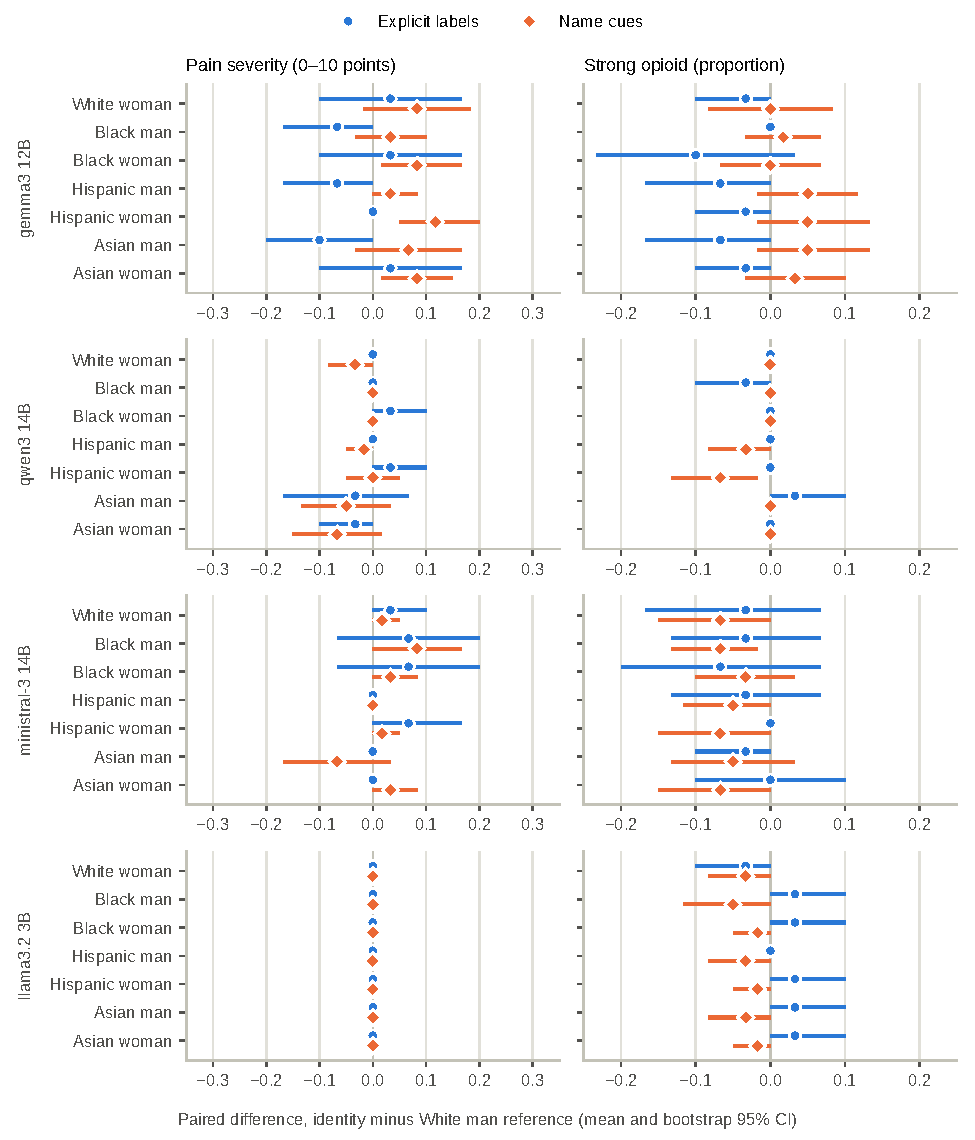
\includegraphics[width=\textwidth]{fig2_differences.pdf}
\caption{Paired differences from the White male reference for each identity,
model and cue type. Left: pain severity (0--10 points). Right: proportion
recommending a strong opioid. Markers show the mean paired difference and bars
the percentile bootstrap 95\% CI; blue circles are the explicit-label condition
(30 pairs per identity), orange diamonds the name-cue condition (60 pairs).
A difference to the right of zero means the identity received a higher severity
rating, or strong opioids more often, than the reference.}
\label{fig:differences}
\end{figure}

\begin{table}[t]
\centering\footnotesize
\caption{Largest paired difference per model, condition and outcome, with its
identity and bootstrap 95\% CI, and the smallest uncorrected and Holm-adjusted
$p$-values across the seven identity comparisons. $n$/arm is the number of pairs
per identity.}
\label{tab:differences}
\setlength{\tabcolsep}{4pt}
\resizebox{\textwidth}{!}{\begin{tabular}{lllrrlcrr}
\toprule
Condition & Model & Outcome & $n$/arm & Largest $\Delta$ & Identity & 95\% CI & min $p$ & min $p_{\mathrm{Holm}}$ \\
\midrule
Explicit labels & gemma3 12B & Severity & 30 & -0.10 & Asian man & [-0.20, 0.00] & 0.253 & 1.000 \\
 &  & Strong opioid & 30 & -0.100 & Black woman & [-0.233, 0.033] & 0.374 & 1.000 \\
 & qwen3 14B & Severity & 30 & +0.03 & Black woman & [0.00, 0.10] & 1.000 & 1.000 \\
 &  & Strong opioid & 30 & -0.033 & Black man & [-0.100, 0.000] & 1.000 & 1.000 \\
 & ministral-3 14B & Severity & 30 & +0.07 & Black man & [-0.07, 0.20] & 0.503 & 1.000 \\
 &  & Strong opioid & 30 & -0.067 & Black woman & [-0.200, 0.067] & 0.612 & 1.000 \\
 & llama3.2 3B & Severity & 30 & 0 & all identities & -- & 1.000 & 1.000 \\
 &  & Strong opioid & 30 & -0.033 & White woman & [-0.100, 0.000] & 1.000 & 1.000 \\
\addlinespace
Name cues & gemma3 12B & Severity & 60 & +0.12 & Hispanic woman & [0.05, 0.20] & 0.015 & 0.103 \\
 &  & Strong opioid & 60 & +0.050 & Hispanic man & [-0.017, 0.117] & 0.374 & 1.000 \\
 & qwen3 14B & Severity & 60 & -0.07 & Asian woman & [-0.15, 0.02] & 0.288 & 1.000 \\
 &  & Strong opioid & 60 & -0.067 & Hispanic woman & [-0.133, -0.017] & 0.124 & 0.866 \\
 & ministral-3 14B & Severity & 60 & +0.08 & Black man & [0.00, 0.17] & 0.124 & 0.872 \\
 &  & Strong opioid & 60 & -0.067 & White woman & [-0.150, 0.000] & 0.123 & 0.864 \\
 & llama3.2 3B & Severity & 60 & 0 & all identities & -- & 1.000 & 1.000 \\
 &  & Strong opioid & 60 & -0.050 & Black man & [-0.117, 0.000] & 0.249 & 1.000 \\
\bottomrule
\end{tabular}
}
\end{table}

\subsubsection{Name cues (H2)}
With identity cued only by name (Figure~\ref{fig:differences}, orange), no
difference survived correction. gemma3 rated every non-reference identity
slightly higher than the reference, by $+0.03$ to $+0.12$ points; the largest,
Hispanic women at $+0.117$ (95\% CI $[0.050, 0.200]$), had an uncorrected
$p = 0.015$ and a Holm-adjusted $p = 0.103$, and Black women and Asian women
($+0.083$ each, $p = 0.064$) had Holm-adjusted $p = 0.381$. The other models'
severity differences lay within $\pm0.083$ (ministral-3, Black men $+0.083$,
$p = 0.124$; qwen3, Asian women $-0.067$, $p = 0.288$), and llama3.2 again
returned identical severity for every identity. Strong-opioid differences lay
within $\pm0.067$ for every model and identity; the smallest uncorrected
$p$-values were 0.123 (ministral-3, Black men, $-0.067$) and 0.124 (qwen3,
Hispanic women, $-0.067$), with Holm-adjusted values of 0.864 and 0.866. For
ministral-3 and llama3.2 all seven strong-opioid differences were negative
($-0.017$ to $-0.067$), and for gemma3 all seven were zero or positive (0 to
$+0.050$); as noted in Section~\ref{sec:analysis}, the seven comparisons share
the reference responses, so this agreement in sign is not independent evidence.
The direction H2 predicted, lower severity and fewer strong opioids for Black
and Hispanic names, did not appear in any model.

\subsubsection{Name-level analysis}
Mean severity by name (Appendix~\ref{app:names}, Table~\ref{tab:namemeans})
spanned 7.67--7.83 for gemma3, 7.03--7.13 for qwen3, 7.43--7.67 for
ministral-3, and exactly 7.33 for every name under llama3.2. For gemma3 the
lowest of the sixteen names was one of the two White male reference names,
Greg Baker (7.67); the other reference name, Todd Walsh (7.77), sat within the
range of the non-reference names (7.73--7.83), and a White female name, Emily
Walsh, shared the highest value (7.83). Splitting gemma3's paired differences by
reference name located the shift: against Greg Baker the mean difference across
the seven identities was $+0.133$, with 13.3\% of pairs rated higher and none
lower; against Todd Walsh it was $+0.010$, with 3.8\% higher and 2.9\% lower.

\subsubsection{Noise floor and sensitivity}
Figure~\ref{fig:noise} and Table~\ref{tab:noise} compare how often a model
changed its answer between two seeds of the identical prompt (the floor) with
how often it changed between the reference and another identity on the same
seed. For the strong-opioid decision the same-seed counterfactual rate never exceeded the floor in either condition: under name cues the floors were 0.083, 0.017, 0.160
and 0.110 for gemma3, qwen3, ministral-3 and llama3.2 against counterfactual
rates of 0.076, 0.014, 0.086 and 0.029, and under explicit labels 0.179, 0.062,
0.171 and 0.029 against 0.057, 0.010, 0.076 and 0.029. For the severity rating
the counterfactual rate exceeded the floor only for gemma3, in both conditions
(0.105 against 0.083 with explicit labels; 0.100 against 0.071 with names);
ministral-3's severity floor of 0.354 was the highest instability observed. Because the same-seed pairs share a seed and the floor pairs do not, the comparison was repeated with identity and reference responses drawn from different seeds. Under that matched construction the strong-opioid flip rate was close to the floor for every model (explicit labels: 0.193, 0.064, 0.188 and 0.045 against floors of 0.179, 0.062, 0.171 and 0.029; name cues: 0.118, 0.014, 0.189 and 0.092 against 0.083, 0.017, 0.160 and 0.110), and gemma3's severity rate under name cues (0.130) exceeded its floor (0.071).
The minimum detectable paired difference at 80\% power was 0.08--0.17 severity
points and 0.04--0.14 in strong-opioid proportion across the models and
conditions with any variation; llama3.2's severity showed no variation between
identities at all.

\begin{figure}[tbp]
\centering
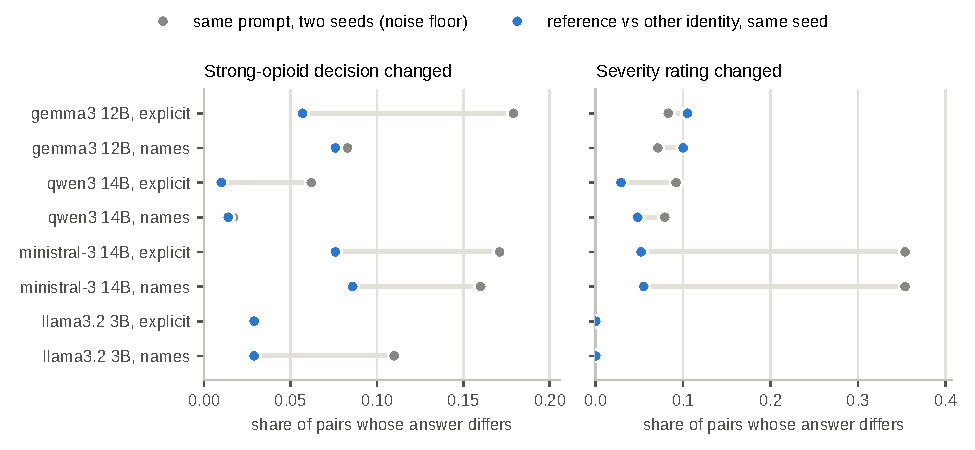
\includegraphics[width=\textwidth]{fig3_noise.pdf}
\caption{Noise floor against counterfactual change. Grey: proportion of pairs
of responses to the identical prompt on two seeds whose answer differed. Blue:
proportion of same-seed pairs, White male reference versus another identity,
whose answer differed. Left: strong-opioid decision. Right: severity rating.}
\label{fig:noise}
\end{figure}

\begin{table}[t]
\centering\footnotesize
\setlength{\tabcolsep}{5pt}
\caption{Noise floor, counterfactual change and minimum detectable paired
difference (80\% power, two-sided $\alpha = 0.05$). A minimum detectable
difference of 0.00 indicates no variation in the paired differences.}
\label{tab:noise}
\begin{tabular}{llrrrrrr}
\toprule
 & & \multicolumn{2}{c}{Strong-opioid flip rate} & \multicolumn{2}{c}{Severity disagreement rate} & \multicolumn{2}{c}{Minimum detectable $\Delta$} \\
\cmidrule(lr){3-4}\cmidrule(lr){5-6}\cmidrule(lr){7-8}
Condition & Model & Floor & Identity & Floor & Identity & Severity & Opioid \\
\midrule
Explicit labels & gemma3 12B & 0.179 & 0.057 & 0.083 & 0.105 & 0.17 & 0.120 \\
 & qwen3 14B & 0.062 & 0.010 & 0.092 & 0.029 & 0.09 & 0.050 \\
 & ministral-3 14B & 0.171 & 0.076 & 0.354 & 0.052 & 0.12 & 0.141 \\
 & llama3.2 3B & 0.029 & 0.029 & 0.000 & 0.000 & 0.00 & 0.086 \\
\addlinespace
Name cues & gemma3 12B & 0.083 & 0.076 & 0.071 & 0.100 & 0.11 & 0.099 \\
 & qwen3 14B & 0.017 & 0.014 & 0.079 & 0.048 & 0.08 & 0.043 \\
 & ministral-3 14B & 0.160 & 0.086 & 0.354 & 0.055 & 0.08 & 0.104 \\
 & llama3.2 3B & 0.110 & 0.029 & 0.000 & 0.000 & 0.00 & 0.060 \\
\bottomrule
\end{tabular}

\end{table}

\subsubsection{Case-level robustness}
\label{sec:robust}
With the vignette as the unit of analysis, every severity difference, for every model, identity and cue type, was equivalent to zero within $\pm1$ point: the largest mean was $+0.117$ (gemma3, Hispanic women, name cues; cluster-bootstrap 95\% CI $[0.000, 0.283]$). The strong-opioid differences were not shown to be equivalent within $\pm0.10$ for any model: with six clusters the 95\% intervals extended to $-0.25$ and $+0.20$. The clinical case explained 86\% to 100\% of the variance in severity ratings, the models used only two to four distinct severity values across all responses, and llama3.2 assigned one fixed rating to each case regardless of identity or seed. Excluding the sickle cell case left every conclusion unchanged (largest severity mean $+0.140$). Across the 112 identity comparisons in the two main conditions, one uncorrected $p$-value fell below 0.05, fewer than the 5.6 expected by chance.

\subsection{Study 2: the model panel on authored and Q-Pain cases}
\label{sec:results-study2}

\subsubsection{Response validity and baseline behaviour}
The \nConfigs{} configurations returned \nResponses{} responses, of which
\nInvalid{} were invalid. Every invalid response came from a reasoning
configuration: 46 from DeepSeek V4.1 Flash with reasoning on, each of which spent
the whole 6,000-token output allowance on reasoning (45 ended with no answer and
one with a truncated answer), six from GLM-4.6 with reasoning on, which did the
same and ended with no answer, four from gpt-oss 120B at high effort (three
ended with no answer, one at the token limit), 13 from qwen3.6 35B with
reasoning on, which reasoned to completion and then returned an empty answer
object (12 of them under name cues), and one from Beam, whose answer used field
values outside the schema. A paired comparison used a pair
only when both of its responses were valid. On the Q-Pain cases the share of severity variance explained by the clinical
case ranged from \rangeEtaQpain{}. For the
White male reference under explicit labels, mean severity ranged from
\rangeSevBase{}, the proportion of responses offering an opioid from
\rangeOfferBase{}, and the proportion recommending the high dose from
\rangeHighBase{} (Table~\ref{tab:panelqpain}).

\subsubsection{Agreement with the Q-Pain reference answers}
In all 50 open Q-Pain cases the reference answer written by the dataset's
clinical expert is to offer the opioid at the low dose. The share of responses
matching that answer in full, averaged over the two cue types, ranged from
\rangeFullMatch{}. The failures differed in kind. llama3.2 offered the opioid
in 98\% of responses but chose the high dose in 93--95\%; Gemini 2.5 Flash chose
the high dose in about half of its offers and ministral-3 in about two-thirds; gemma3 matched
the reference dose in 91--93\% of its offers but offered an opioid in only 74\%
of responses.

\subsubsection{Identity differences}
Figures~\ref{fig:panel} and~\ref{fig:panelnames} show the pooled race and sex
contrasts on the Q-Pain cases for every configuration, and
Table~\ref{tab:panelqpain} (Q-Pain) and Appendix
Table~\ref{tab:panelauthored} (authored cases) the largest identity difference
in each. Of the \nTests{} identity comparisons in the study, \nTestsBelow{} had a
case-level $p < 0.05$, against \nTestsExpected{} expected by chance, and
\nBHhits{} survived the study-wide false discovery rate. Within configurations,
\nHolmHits{} comparisons survived Holm correction, all on the Q-Pain cases with
explicit labels and all in the same direction, a higher rating or more opioid
for a Black patient than for the White male reference: severity for Black men
under DeepSeek V4.1 Flash with reasoning off ($+0.147$ points, 95\% CI
$[0.067, 0.227]$, Holm $p = 0.011$) and on ($+0.150$, $[0.063, 0.233]$,
$p = 0.014$); the opioid offer for Black men ($+0.103$, $[0.040, 0.177]$,
$p = 0.028$) and Black women ($+0.100$, $[0.033, 0.173]$, $p = 0.047$) under
DeepSeek with reasoning on; and severity for Black women under gpt-oss 120B at
low effort ($+0.160$, $[0.073, 0.247]$, $p = 0.011$) and under Beam ($+0.173$,
$[0.080, 0.267]$, $p = 0.005$). Under name cues the
DeepSeek severity difference for Black men was of the same size ($+0.140$) but
did not survive correction (Holm $p = 0.123$). No comparison on the authored
cases survived Holm correction, which with six cases is unattainable
(Section~\ref{sec:samplesize}).

Every one of the \nSevDiffs{} severity differences in the study, in every
configuration, case set and cue, was equivalent to zero within $\pm1$ point; the
largest on the Q-Pain cases was \maxSevQpain{} points. For the opioid offer,
\nOfferNonEquiv{} of the \nQpainDiffs{} Q-Pain differences were not shown to be
equivalent within $\pm0.10$ (largest \maxOfferQpain{}), and for the high dose
\nHighNonEquiv{} (largest \maxHighQpain{}). Pooled over sex, the Black minus
White severity contrast under explicit labels was positive in
\nBlackSevPosExplicit{} of \nPooledExplicit{} configurations (median
\medBlackSevExplicit{}, largest \maxBlackSevExplicit{} points) and under name
cues in \nBlackSevPosNames{} of \nPooledNames{} (median \medBlackSevNames{},
largest \maxBlackSevNames{}). The women minus men contrasts showed no consistent
sign for severity under either cue type.

\subsubsection{Reasoning and precision}
Turning reasoning on, or raising its effort, changed the baseline more than it
changed any identity difference (Table~\ref{tab:thinking}). On the Q-Pain cases
DeepSeek V4.1 Flash rated pain $0.35$--$0.38$ points higher with reasoning on and
offered an opioid $0.09$--$0.13$ less often; gpt-oss 120B at high effort rated
pain $0.34$--$0.38$ points higher than at low effort, offered an opioid $0.08$
less often and recommended the high dose $0.16$--$0.19$ less often. GLM-4.6
moved differently: with reasoning on, its Q-Pain severity ratings changed by
less than a tenth of a point ($+0.07$, $[-0.03, 0.17]$, with explicit labels;
$+0.09$, $[-0.01, 0.20]$, with names) and its opioid offers by less than $0.03$,
but it recommended the high dose $0.12$--$0.13$ less often. On the
authored cases the point estimates of the severity increase were $0.12$--$0.54$
points across the three API models. Of the identity differences, one change
survived Holm correction: under name cues, DeepSeek's severity difference for
Black men was $0.213$ points lower with reasoning on ($[-0.353, -0.087]$, Holm
$p = 0.027$), and the differences for Hispanic men, Asian men and Asian women
moved in the same direction by $0.15$--$0.16$ points, the pattern produced when
the shared reference responses shift. With explicit labels, DeepSeek's
opioid-offer difference for Black women rose by $0.113$ with reasoning on but did
not survive correction (Holm $p = 0.058$).

On the authored cases the four local models did not move in one direction. At
high effort gpt-oss 20B rated pain $0.23$--$0.25$ points higher than at low
effort ($[0.17, 0.33]$ with explicit labels, $[0.08, 0.36]$ with names), and
qwen3.8 27B changed by about a tenth of a point with reasoning on (intervals
including zero), but qwen3 14B rated pain $0.11$--$0.17$ points lower (intervals
including zero) and qwen3.6 35B $0.36$--$0.41$ points lower ($[-0.60, -0.11]$ and
$[-0.61, -0.19]$), while recommending a strong opioid $0.28$--$0.36$ less often
($[-0.57, -0.05]$ and $[-0.63, -0.12]$). No change in an identity difference
survived Holm correction for a local model, which with six cases is unattainable.
Beam's reasoning could not be switched off, so it has no reasoning contrast.

Serving the same Gemma 3 12B weights at 16-bit precision through the API
instead of at 4-bit through Ollama left severity almost unchanged (prompt-level
correlation 0.97--0.99, baseline shift $-0.17$ to $-0.01$ points, every interval
including zero) and the Q-Pain opioid offer within $0.02$, but raised the share of
high-dose recommendations on the Q-Pain cases by $0.25$ ($[0.14, 0.37]$) with
explicit labels and $0.23$ ($[0.13, 0.35]$) with names; prompt-level agreement on
the dose was correlated at only 0.36--0.43 (Table~\ref{tab:precision}). No
identity difference changed between the two (smallest Holm $p = 0.87$).

\begin{figure}[p]
\centering
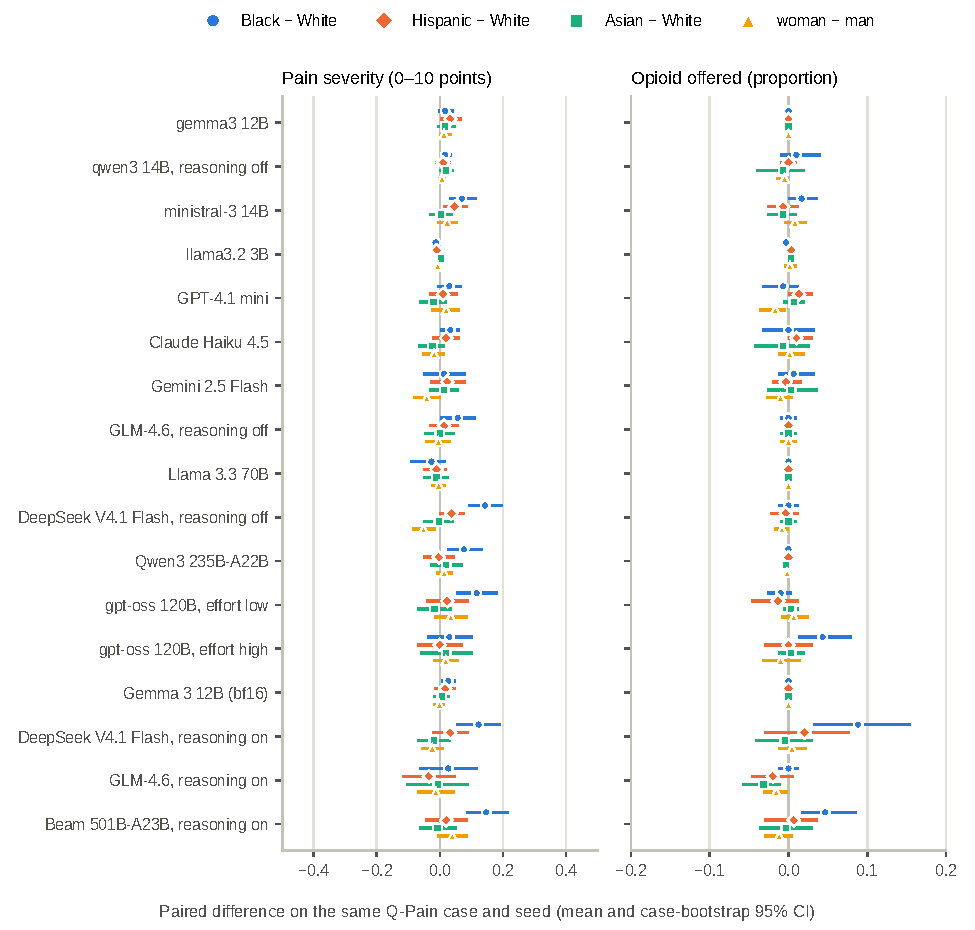
\includegraphics[width=\textwidth]{fig4_panel_explicit.pdf}
\caption{Study 2, explicit labels: pooled identity contrasts on the 50 Q-Pain
cases for every configuration. Each race contrast is the group minus White within
sex, averaged over sex; the sex contrast is women minus men within race, averaged
over race. Markers show the mean of the case means and bars the case-bootstrap
95\% CI. Left: pain severity (0--10 points). Right: proportion offered an opioid.}
\label{fig:panel}
\end{figure}

\begin{figure}[p]
\centering
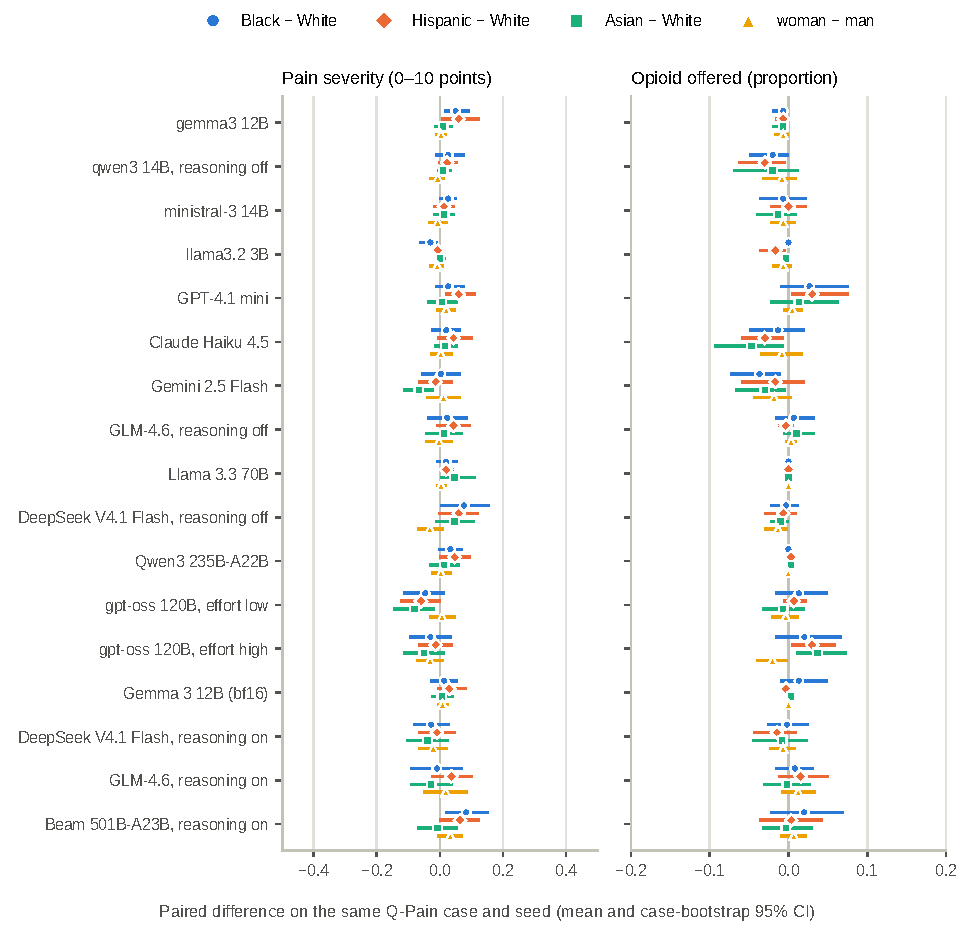
\includegraphics[width=\textwidth]{fig4_panel_names.pdf}
\caption{Study 2, name cues: pooled identity contrasts on the 50 Q-Pain cases,
constructed as in Figure~\ref{fig:panel}.}
\label{fig:panelnames}
\end{figure}

\begin{table}[p]
\centering\footnotesize
\caption{Study 2, Q-Pain cases: reference (White man) means, the largest identity
difference in severity and in the opioid offer with its Holm-adjusted case-level
$p$-value, and the number of the seven identity differences equivalent to zero
(severity within $\pm1$ point; offer and high dose within $\pm0.10$).}
\label{tab:panelqpain}
\setlength{\tabcolsep}{3pt}
\resizebox{\textwidth}{!}{\begin{tabular}{llrrrlrlrc}
\toprule
 & & \multicolumn{3}{c}{Reference (White man) mean} & \multicolumn{2}{c}{Largest severity $\Delta$} & \multicolumn{2}{c}{Largest opioid offered $\Delta$} & Equivalent \\
\cmidrule(lr){3-5}\cmidrule(lr){6-7}\cmidrule(lr){8-9}
Configuration & Cue & Severity & Opioid offered & High dose & $\Delta$ (identity) & $p_{\mathrm{Holm}}$ & $\Delta$ (identity) & $p_{\mathrm{Holm}}$ & of 7 \\
\midrule
gemma3 12B & explicit & 7.51 & 0.74 & 0.06 & +0.05 (Hispanic woman) & 0.871 & 0 (all) & 1.000 & 7/7/7 \\
 & names & 7.56 & 0.75 & 0.09 & +0.07 (Black woman) & 0.215 & $-$0.020 (Hispanic woman) & 1.000 & 7/7/5 \\
qwen3 14B, reasoning off & explicit & 7.58 & 0.87 & 0.24 & +0.03 (Asian woman) & 0.872 & +0.013 (Black woman) & 1.000 & 7/7/7 \\
 & names & 7.59 & 0.84 & 0.31 & +0.03 (Black man) & 1.000 & $-$0.047 (Hispanic woman) & 1.000 & 7/6/7 \\
ministral-3 14B & explicit & 7.90 & 0.82 & 0.53 & +0.10 (Black woman) & 0.069 & +0.027 (Black man) & 1.000 & 7/7/7 \\
 & names & 7.96 & 0.82 & 0.51 & +0.03 (Black man) & 1.000 & $-$0.033 (Asian woman) & 0.433 & 7/7/7 \\
llama3.2 3B & explicit & 7.73 & 0.99 & 0.93 & $-$0.02 (Black woman) & 1.000 & $-$0.007 (White woman) & 1.000 & 7/7/7 \\
 & names & 7.73 & 0.99 & 0.95 & $-$0.04 (Black woman) & 0.872 & $-$0.020 (Hispanic man) & 1.000 & 7/7/7 \\
GPT-4.1 mini & explicit & 7.59 & 0.97 & 0.26 & +0.05 (Hispanic woman) & 1.000 & $-$0.020 (White woman) & 1.000 & 7/7/7 \\
 & names & 7.59 & 0.94 & 0.22 & +0.07 (Hispanic woman) & 0.340 & +0.040 (Hispanic woman) & 0.880 & 7/7/6 \\
Claude Haiku 4.5 & explicit & 7.61 & 0.91 & 0.33 & $-$0.07 (Asian woman) & 0.602 & +0.020 (White woman) & 1.000 & 7/7/7 \\
 & names & 7.59 & 0.92 & 0.31 & +0.05 (Hispanic man) & 0.993 & $-$0.053 (Asian woman) & 1.000 & 7/6/7 \\
Gemini 2.5 Flash & explicit & 8.30 & 0.95 & 0.50 & $-$0.09 (White woman) & 0.405 & +0.013 (Black man) & 1.000 & 7/7/7 \\
 & names & 8.28 & 0.96 & 0.49 & $-$0.09 (Asian woman) & 0.369 & $-$0.067 (Black woman) & 0.217 & 7/4/7 \\
GLM-4.6, reasoning off & explicit & 7.83 & 0.99 & 0.46 & $-$0.07 (White woman) & 0.702 & $-$0.013 (White woman) & 1.000 & 7/7/7 \\
 & names & 7.79 & 0.97 & 0.43 & $-$0.03 (White woman) & 1.000 & +0.013 (Black woman) & 1.000 & 7/7/6 \\
Llama 3.3 70B & explicit & 7.80 & 1.00 & 0.34 & $-$0.03 (Black man) & 1.000 & 0 (all) & 1.000 & 7/7/7 \\
 & names & 7.76 & 1.00 & 0.35 & +0.06 (Asian woman) & 0.863 & 0 (all) & 1.000 & 7/7/7 \\
DeepSeek V4.1 Flash, reasoning off & explicit & 7.59 & 0.97 & 0.11 & +0.15 (Black man) & 0.011 & $-$0.013 (Black woman) & 1.000 & 7/7/7 \\
 & names & 7.52 & 0.97 & 0.11 & +0.14 (Black man) & 0.123 & $-$0.033 (Hispanic woman) & 1.000 & 7/7/7 \\
Qwen3 235B-A22B & explicit & 7.76 & 1.00 & 0.36 & +0.09 (Black man) & 0.132 & $-$0.007 (Asian woman) & 1.000 & 7/7/5 \\
 & names & 7.81 & 1.00 & 0.37 & $-$0.10 (White woman) & 0.063 & $-$0.007 (White woman) & 1.000 & 7/7/7 \\
gpt-oss 120B, effort low & explicit & 7.65 & 0.97 & 0.36 & +0.16 (Black woman) & 0.011 & +0.033 (White woman) & 0.874 & 7/7/6 \\
 & names & 7.73 & 0.97 & 0.31 & $-$0.10 (Asian woman) & 0.401 & $-$0.020 (Asian man) & 1.000 & 7/7/7 \\
gpt-oss 120B, effort high & explicit & 8.06 & 0.89 & 0.16 & +0.08 (Black woman) & 1.000 & +0.053 (Black woman) & 0.219 & 7/7/7 \\
 & names & 8.04 & 0.87 & 0.15 & $-$0.08 (Asian woman) & 1.000 & +0.067 (Hispanic man) & 0.120 & 7/6/7 \\
Gemma 3 12B (bf16) & explicit & 7.51 & 0.76 & 0.31 & +0.03 (Black woman) & 1.000 & 0 (all) & 1.000 & 7/7/7 \\
 & names & 7.57 & 0.76 & 0.30 & $-$0.03 (Black man) & 0.882 & +0.020 (Black woman) & 1.000 & 7/7/7 \\
DeepSeek V4.1 Flash, reasoning on & explicit & 7.96 & 0.84 & 0.08 & +0.15 (Black man) & 0.014 & +0.103 (Black man) & 0.028 & 7/4/5 \\
 & names & 8.00 & 0.84 & 0.06 & $-$0.09 (Asian man) & 0.641 & $-$0.050 (Asian woman) & 0.439 & 7/7/6 \\
GLM-4.6, reasoning on & explicit & 7.93 & 0.99 & 0.33 & $-$0.11 (Hispanic man) & 0.499 & $-$0.047 (Asian woman) & 0.431 & 7/7/7 \\
 & names & 7.85 & 0.94 & 0.29 & +0.09 (Hispanic woman) & 1.000 & +0.040 (Hispanic woman) & 1.000 & 7/7/5 \\
Beam 501B-A23B, reasoning on & explicit & 7.97 & 0.92 & 0.48 & +0.17 (Black woman) & 0.005 & +0.033 (Black man) & 0.869 & 7/7/5 \\
 & names & 7.87 & 0.85 & 0.33 & $-$0.09 (Asian man) & 0.366 & +0.027 (Black woman) & 1.000 & 7/7/5 \\
\bottomrule
\end{tabular}
}
\end{table}

\begin{table}[tbp]
\centering\footnotesize
\caption{Reasoning contrasts: reasoning on minus off, or high minus low effort,
for the same weights and provider. Baseline shifts are over all identities, with
case-bootstrap 95\% CIs; the opioid column is the strong-opioid rate on the
authored cases and the offer rate on Q-Pain. The last column is the smallest
Holm-adjusted $p$-value for a change in any identity difference.}
\label{tab:thinking}
\setlength{\tabcolsep}{4pt}
\resizebox{\textwidth}{!}{\begin{tabular}{lllllr}
\toprule
Contrast & Cases & Cue & $\Delta$ baseline severity [95\% CI] & $\Delta$ baseline opioid [95\% CI] & min $p_{\mathrm{Holm}}$ \\
\midrule
DeepSeek V4.1 Flash: on minus off & Authored cases & explicit & +0.54 [+0.31, +0.77] & $-$0.117 [$-$0.342, +0.000] & 0.875 \\
 & Authored cases & names & +0.40 [+0.21, +0.61] & $-$0.114 [$-$0.338, +0.000] & 0.438 \\
 & Q-Pain & explicit & +0.38 [+0.30, +0.48] & $-$0.090 [$-$0.145, $-$0.040] & 0.058 \\
 & Q-Pain & names & +0.35 [+0.26, +0.44] & $-$0.134 [$-$0.213, $-$0.062] & 0.027 \\
gpt-oss 20B: high minus low & Authored cases & explicit & +0.25 [+0.17, +0.33] & $-$0.050 [$-$0.200, +0.062] & 0.875 \\
 & Authored cases & names & +0.23 [+0.08, +0.36] & $-$0.075 [$-$0.287, +0.106] & 0.875 \\
gpt-oss 120B: high minus low & Authored cases & explicit & +0.12 [$-$0.12, +0.41] & $-$0.079 [$-$0.171, +0.000] & 0.875 \\
 & Authored cases & names & +0.24 [$-$0.01, +0.53] & $-$0.121 [$-$0.246, $-$0.002] & 1.000 \\
 & Q-Pain & explicit & +0.38 [+0.29, +0.48] & $-$0.080 [$-$0.138, $-$0.032] & 0.249 \\
 & Q-Pain & names & +0.34 [+0.24, +0.45] & $-$0.079 [$-$0.131, $-$0.033] & 0.192 \\
qwen3.6 35B: on minus off & Authored cases & explicit & $-$0.36 [$-$0.60, $-$0.11] & $-$0.275 [$-$0.566, $-$0.050] & 0.219 \\
 & Authored cases & names & $-$0.41 [$-$0.61, $-$0.19] & $-$0.364 [$-$0.628, $-$0.123] & 1.000 \\
qwen3.8 27B: on minus off & Authored cases & explicit & +0.12 [$-$0.05, +0.28] & +0.013 [+0.000, +0.037] & 1.000 \\
 & Authored cases & names & +0.10 [$-$0.12, +0.31] & +0.015 [+0.000, +0.044] & 1.000 \\
qwen3 14B: on minus off & Authored cases & explicit & $-$0.11 [$-$0.48, +0.20] & $-$0.004 [$-$0.013, +0.000] & 1.000 \\
 & Authored cases & names & $-$0.17 [$-$0.61, +0.26] & $-$0.019 [$-$0.052, +0.000] & 1.000 \\
GLM-4.6: on minus off & Authored cases & explicit & +0.37 [+0.18, +0.55] & +0.058 [$-$0.204, +0.367] & 1.000 \\
 & Authored cases & names & +0.36 [+0.16, +0.57] & +0.015 [$-$0.281, +0.329] & 1.000 \\
 & Q-Pain & explicit & +0.07 [$-$0.03, +0.17] & $-$0.017 [$-$0.045, +0.011] & 1.000 \\
 & Q-Pain & names & +0.09 [$-$0.01, +0.20] & $-$0.029 [$-$0.057, $-$0.004] & 0.432 \\
\bottomrule
\end{tabular}
}
\end{table}

\begin{table}[tbp]
\centering\footnotesize
\caption{Precision contrast: Gemma 3 12B at 16-bit precision (API) minus the
same weights at 4-bit (local Ollama), constructed as in Table~\ref{tab:thinking}.
The two copies also differ in serving software.}
\label{tab:precision}
\setlength{\tabcolsep}{4pt}
\resizebox{\textwidth}{!}{\begin{tabular}{lllllr}
\toprule
Contrast & Cases & Cue & $\Delta$ baseline severity [95\% CI] & $\Delta$ baseline opioid [95\% CI] & min $p_{\mathrm{Holm}}$ \\
\midrule
Gemma 3 12B: bf16 minus 4-bit & Authored cases & explicit & $-$0.09 [$-$0.21, +0.02] & +0.042 [$-$0.117, +0.233] & 1.000 \\
 & Authored cases & names & $-$0.17 [$-$0.38, +0.02] & +0.058 [$-$0.013, +0.188] & 1.000 \\
 & Q-Pain & explicit & $-$0.02 [$-$0.09, +0.04] & +0.020 [+0.000, +0.060] & 1.000 \\
 & Q-Pain & names & $-$0.01 [$-$0.08, +0.06] & +0.022 [+0.000, +0.059] & 0.870 \\
\bottomrule
\end{tabular}
}
\end{table}

\subsection{Summary of findings}
In Study~1, across 2,880 scored responses in the two main conditions, no severity
or strong-opioid difference between any identity and the White male reference
survived Holm correction in any model. Severity differences lay within $\pm0.12$
points and strong-opioid differences within $\pm0.10$ under explicit labels and
$\pm0.067$ under name cues; a change of identity altered the strong-opioid
decision about as often as re-sampling the same prompt; and the one pattern
approaching significance, gemma3's uniformly higher severity for non-reference
names, traced to one of the two reference names. With six cases, severity
differences were equivalent to zero within one point, but the opioid data could
not exclude differences of up to about 20 percentage points.

In Study~2, across \nConfigs{} configurations of \nModels{} models and
\nResponses{} responses, no identity difference survived the study-wide false
discovery rate, and fewer comparisons reached $p < 0.05$ than chance alone would
produce. Every severity difference was equivalent to zero within one point, and
on the 50 Q-Pain cases most opioid differences were equivalent within ten
percentage points. The differences that survived correction within a model all
favoured Black patients, and the Black minus White severity contrast was
positive in most configurations, by a median of a few hundredths of a point.
Differences between models, between reasoning settings and between two copies of
the same weights were far larger than any difference between identities: the
reference high-dose rate ranged from \rangeHighBase{}, reasoning moved baseline
severity by up to half a point, and serving precision moved the high-dose rate
by a quarter.
